
\documentclass[]{report}

\voffset=-1.5cm
\oddsidemargin=0.0cm
\textwidth = 480pt

\usepackage{framed}
\usepackage{subfiles}
\usepackage{graphics}
\usepackage{newlfont}
\usepackage{eurosym}
\usepackage{amsmath,amsthm,amsfonts}
\usepackage{amsmath}
\usepackage{enumerate}
\usepackage{color}
\usepackage{multicol}
\usepackage{amssymb}
\usepackage{multicol}
\usepackage[dvipsnames]{xcolor}
\usepackage{graphicx}
\begin{document}

% \maketitle


\subsection*{Operations Research - Tutorial Set Question 1 to 30}

\begin{enumerate}
	\item 
	Find a solution to each game, i.e, an optimum strategy $p^o$ for R, an optimum strategy $q^o$ for C, and the value of the game. 
\begin{figure}[h!]
\centering
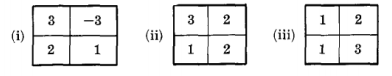
\includegraphics[width=0.55\linewidth]{TutQ1}
%\caption{}
\label{fig:tutq1}
\end{figure}
\begin{itemize}
\item \textit{Identify the saddle point and value of a Strictly Determined Game (Week 1)}


\end{itemize}
	\item 
	Which of the following games are strictly determined ? For the strictly determined games, find the value v of the game and find an optimum strategy $p^o$  for the row player R and an optimum strategy $q^o$  for the column player C. 
	
\begin{figure}[h!]
	\centering
	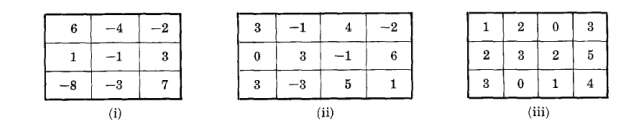
\includegraphics[width=0.8\linewidth]{TutQ2}
	%\caption{}
	\label{fig:tutq2}
\end{figure}
	
	\item 

	Find the solution to each of the following 2 x 2 games. 
\begin{figure}[h!]
	\centering
	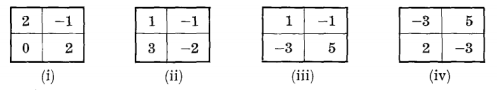
\includegraphics[width=0.65\linewidth]{TutQ3}
	%\caption{}
	\label{fig:tutq3}
\end{figure}

	
	\item Two players R and C simultaneously show 2 or 3 fingers. If the sum of the fingers shown is even, then R wins the sum from C; if the sum is odd, then R loses the sum to C. Find optimum strategies for the players and to whom the game is favorable. 
	
	\item 
	Find the solution to the following game 
\begin{figure}[h!]
	\centering
	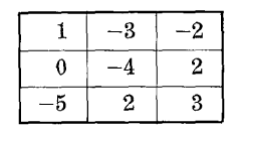
\includegraphics[width=0.35\linewidth]{TutQ5}
	%\caption{}
	\label{fig:tutq5}
\end{figure}

%===========================%
\item Identify optimal strategy profiles and value of a non-strictly determined game.
\begin{itemize}
	
	\item \textit{Similar to Question 3}
	
\end{itemize}
%===========================%
\item Statement of a game matrix, given a scenario.
\begin{itemize}
	
	\item \textit{See Week 5 handout 2 - Amy and Beth Example}
	
\end{itemize}
\item Questions on Iterative Elimination of Dominated Strategies 
\begin{itemize}
\item \textit{Zero Sum Games - expect to reduce to a ``2 by 2" or ``2 by 3"}
\item \textit{Show your workings. Expect one or two such matrices}
\end{itemize}
\item Short definition of Nash Equilibrium
\item \textbf{\textit{Worked Example of Nash Equilibrium}}\\
Determine the Nash Equilibrium of the following game.

\begin{center}
	\begin{tabular}{|c|c|c|} \hline 
		&    L    & R \\ \hline 
		T  &    (1,1)    & (6,-2) \\ \hline
		M  &   (-2,6)    &  (3,3) \\ \hline
	\end{tabular}
\end{center}

	
%===========================%
\item Essay Question about Prisoner's Dilemma
\begin{itemize}
\item \textit{Include a relevant Pay-off matrix}
\item \textit{Discuss Nash Equilibrium}
\end{itemize}
%===========================%
\item Describe a graphical method for presenting extensive form games.

\begin{itemize}

\item \textit{Kuhn Trees - from Week 5 handout 1}

\end{itemize}

\item Depict the following matrix game as an extensive form game. You may assume that Player 1 moves first, and Player 2 reacts.

\begin{center}
\begin{tabular}{|c|c|c|c|} \hline 
   &    L  &  C  & R \\ \hline 
T  &    6  &  -7  & -3 \\ \hline
B  &   -6  &   5  &  4 \\ \hline
\end{tabular}
\end{center}
\begin{itemize}
	
	\item \textit{See Week 5 handout 1}
	
\end{itemize}
%===========================%
% Question 14
\item Design a binary search tree for an ordered list of 17,21 and 30 Records. For each case, what is the maximum number of comparisons that the computer would have to make to match any existing record?

% Question 15
\item A mail order company has 5,000,000 records on its database. Calculate the maximum number of comparisons that would need to be made to match a target with any record in the database. 
\begin{itemize}

\item \textit{For last two questions - see Week 3 handout}
%\item \textit{See Questions at end of handout , i.e. Q7 and Q8}
\end{itemize}
%===========================%
% Question 16
\item  Consider the following game. Player 1 moves first and can take action A or B.
 Player 2 observes the action of Player 1 and independently of the action of Player 1 can
 take action A or B. If both play A, then Player 1 obtains a payoff of 4 and Player 2
 obtains a payoff of 5. If Player 1 plays A and Player 2 plays B, then Player 1 obtains a
 payoff of 2 and Player 2 obtains a payoff of 7. If Player 1 plays B and Player 2 plays A,
 then Player 1 obtains a payoff of 6 and Player 2 obtains a payoff of 3. If both play B,
 then Player 1 obtains a payoff of 0 and Player 2 obtains a payoff of 1.
\begin{enumerate}[(a)]
\item Draw the tree depicting the extensive form of the game.
\item Solve the game using recursion.
\item Give the matrix form of the game.
\end{enumerate} 
\smallskip
\begin{itemize}
	
	\item \textit{See Week 5 handout 2}
	
\end{itemize}
%==================================%
%- Question 17
\item Consider the following matrix game. Find the minimax solution of this game.
\begin{center}
	\begin{tabular}{|c|c|c|} \hline   & A & B\\ \hline
 A &(4,5)& (2,7)\\ \hline
 B & (6,3)& (0,1)\\ \hline
\end{tabular}
\end{center}

%==================================%
%- Question 18

\item By removing all strategies which are dominated by pure or mixed strategies,
derive the reduced version of the following matrix game.
\begin{center}
	\begin{tabular}{|c|c|c|c|c|} \hline 
   & D & E & F & G \\ \hline
A & (5,2)& (2,4) & (3,3) & (4,4) \\ \hline
B & (3,3)& (5,2) & (3,5) & (2,3) \\ \hline
C & (4,4)& (4,6) & (4,3) & (5,4) \\ \hline
\end{tabular}
\end{center}
\begin{enumerate}[(a)]
	\item Derive the minimax solution of this game.
%	\item Derive the Nash equilibria and values of this game.
\end{enumerate}
%==================================%
%- Question 19

\item 
Reduce the following bimatrix by
\begin{enumerate}[(a)]
	\item Iterative Elimination of Strongly Dominated Strategies (IESDS)
	\item Iterative Elimination of Weakly Dominated Strategies (IEWDS)
\end{enumerate}
%\begin{itemize}
%	\item (See \textit{See Question 19.})
%\end{itemize}
\begin{center}
	\begin{tabular}{|c|c|c|c|} \hline 
		&    L  &  C  & R \\ \hline 
		T  &   (3,2) &  (3,2) &  (2,3) \\ \hline
     	M  &    (3,2)  &   (2,3)  &  (1.1) \\ \hline
		B  &    (2,3)  &    (1,1)  &   (1,1) \\ \hline
	\end{tabular}
\end{center}
%==================================%
%- Question 19
\item State the weakly dominated strategy equilibrium for both games below
\begin{figure}[h!]
\centering
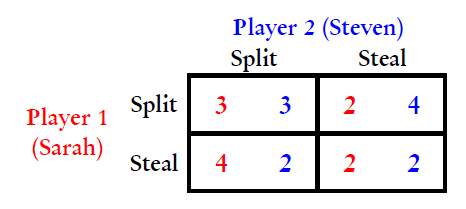
\includegraphics[width=0.45\linewidth]{Question20}
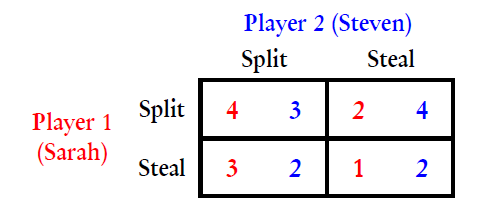
\includegraphics[width=0.45\linewidth]{Question20-b}
\end{figure}
	
\newpage	
%===========================%
% Question 21
 \item
 \begin{enumerate}[(a)]
 	
 	
 	\item Provide a short description of the Dynamic Programing Paradigm.  
 	\item What is a Greedy Algorithm? Support your answer with a simple example, and discuss the advantages and disadvantages of using Greedy Algorithms.   														
 	\item In the context of the design of algorithms, describe the Divide and Conquer paradigm.
 \end{enumerate}
 
 


%===========================%
% Question 22
\item Minimax Question 
\begin{itemize}
	
	\item Short Definition
	\item Worked Example - See Handouts and Question 29
\end{itemize}
%===========================%
% Question 23
\item \textbf{\textit{Short Game Theory Questions}} : Provide Short definitions of the following.
\begin{itemize}
	
	\item Perfect Information
	\item Assumption of Rationality
	\item Pareto Optimality
\end{itemize}
%===========================%
%- Question 24
\item Linear Programming (LP) Solution
\begin{itemize}
	
	\item \textit{This will be part of IP Branch and Bound Question later in course.}

\end{itemize}
%===========================%
%- Question 25
\item Explain the difference between Linear Programming (LP) and Integer Programming (IP). Explain what is meant by LP Relaxation.
\begin{itemize}
	
	\item \textit{This will be part of IP Branch and Bound Question later in course.}
	
\end{itemize}
%======================%
% Question 26

\item Apply the IDSDS procedure to the following game. Is there a strict
iterated dominant-strategy equilibrium? \begin{figure}[h!]
\centering
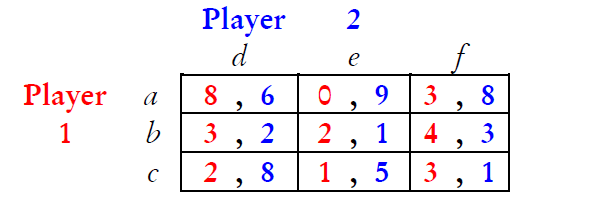
\includegraphics[width=0.55\linewidth]{Question26}
\end{figure}
\begin{itemize}
	\item \textit{See Question 19.}
\end{itemize}

%======================%
% Question 27
\newpage
\item Consider the following game: \begin{figure}[h!]
	\centering
	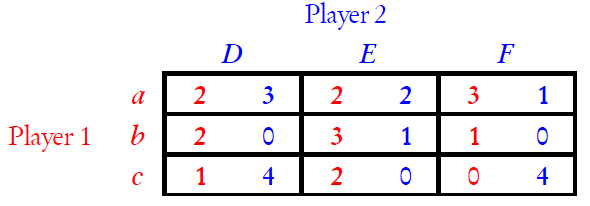
\includegraphics[width=0.45\linewidth]{Question27}
\end{figure}
\begin{enumerate}[(a)]
\item Apply the IDSDS procedure to it. Is there an iterated strict dominant-strategy
equilibrium?
\item  Apply the IDWDS procedure to it. Is there an iterated weak dominant-strategy
equilibrium?
\end{enumerate}

\begin{itemize}
	\item \textit{See Question 19 and 26.}
	
\end{itemize}	
\item \textit{Statement of a Simplex Tableau to solve a Game Theory Problem}
%=========================%
\item By removing all strategies which are dominated by pure or mixed strategies,
derive the reduced version of the following matrix game. Then derive the minimax solution of this game.

\begin{center}
	\begin{tabular}{|c|c|c|c|} \hline 
		&    L  &  C  & R \\ \hline 
		T  &   3 &  -2 &  2 \\ \hline
		M  &    -1  &   0  &  4 \\ \hline
		B  &   -4  &    -3  &   1 \\ \hline
	\end{tabular}
\end{center}
%=========================%

%- Question 30
\item Express the following Kuhn Tree in matrix form. 
Use Backward Induction to state an equilibrium solution.
\begin{figure}[h!]
\centering
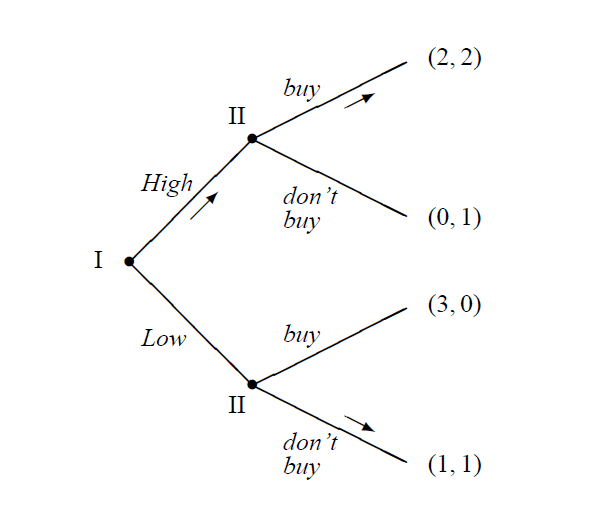
\includegraphics[width=0.4\linewidth]{Q30}

\end{figure}
\end{enumerate}

\end{document}
